\section{Stable Diffusion Core Backbone: Attention-U-Net Architecture}

\begin{frame}[plain]
    \centering
    \vspace{2cm}
    {\Huge \textcolor{blue}{Stable Diffusion Core Backbone:}\\[1em]
     \textbf{Attention-U-Net Architecture}}
\end{frame}

\newcommand{\binxuwSdCaption}{%
  {\scriptsize Binxu Wang \& John Vastola, \href{https://binxuw.scholars.harvard.edu/sites/g/files/omnuum11221/files/binxuw/files/stable_diffusion_a_tutorial.pdf}{Stable Diffusion: A Tutorial (Harvard ML from Scratch)}, 2022.}%
}

\begin{frame}{Refresher: Convolutional Neural Network}
  \begin{columns}[T,onlytextwidth]
    \column{0.48\textwidth}
      \begin{itemize}\itemsep0.35em\footnotesize
        \item CNN parametrizes a function over images.
        \item \textbf{Motivation:}
        \begin{itemize}
          \item Features are translationally invariant.
          \item Extract features at different scales / abstraction levels.
        \end{itemize}
        \item \textbf{Key modules:}
        \begin{itemize}
          \item Convolution
          \item Downsampling (max-pool)
        \end{itemize}
        \item Features of larger scale (larger receptive field) $\Rightarrow$ higher abstraction level.
      \end{itemize}
    \column{0.50\textwidth}
      \centering
      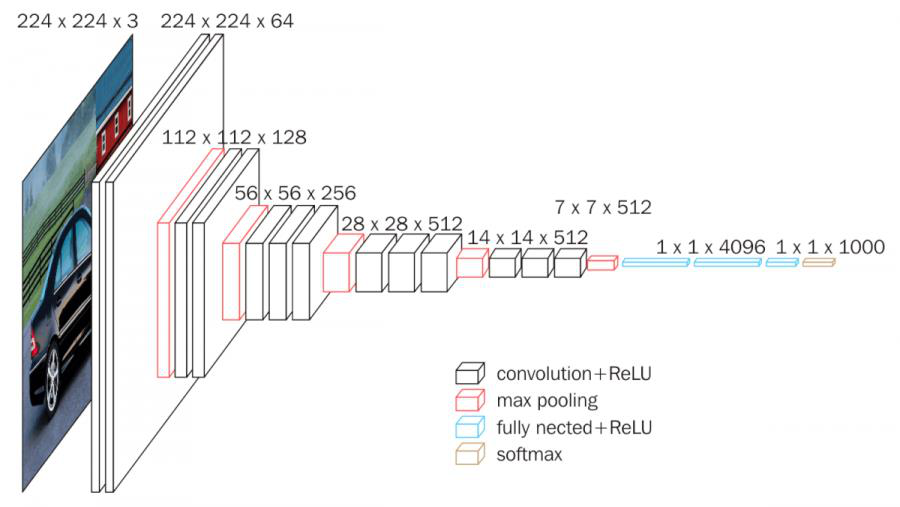
\includegraphics[width=\linewidth,height=0.72\textheight,keepaspectratio]{images/stable-diffusion/cnn_refresher.png}\\[0.25em]
      \binxuwSdCaption
  \end{columns}
\end{frame}

\begin{frame}{CNN + inverted CNN $\Rightarrow$ U-Net}
      \begin{itemize}
        \item An inverted CNN (generator) can generate images.
        \item CNN + inverted CNN can model an image-to-image function.
        \item \textbf{Down sampling:} convolution.
        \item \textbf{Up sampling:} transposed convolution.
      \end{itemize}
\end{frame}

\begin{frame}{U-Net: A Natural Architecture for Image-to-Image Functions}
    \centering
    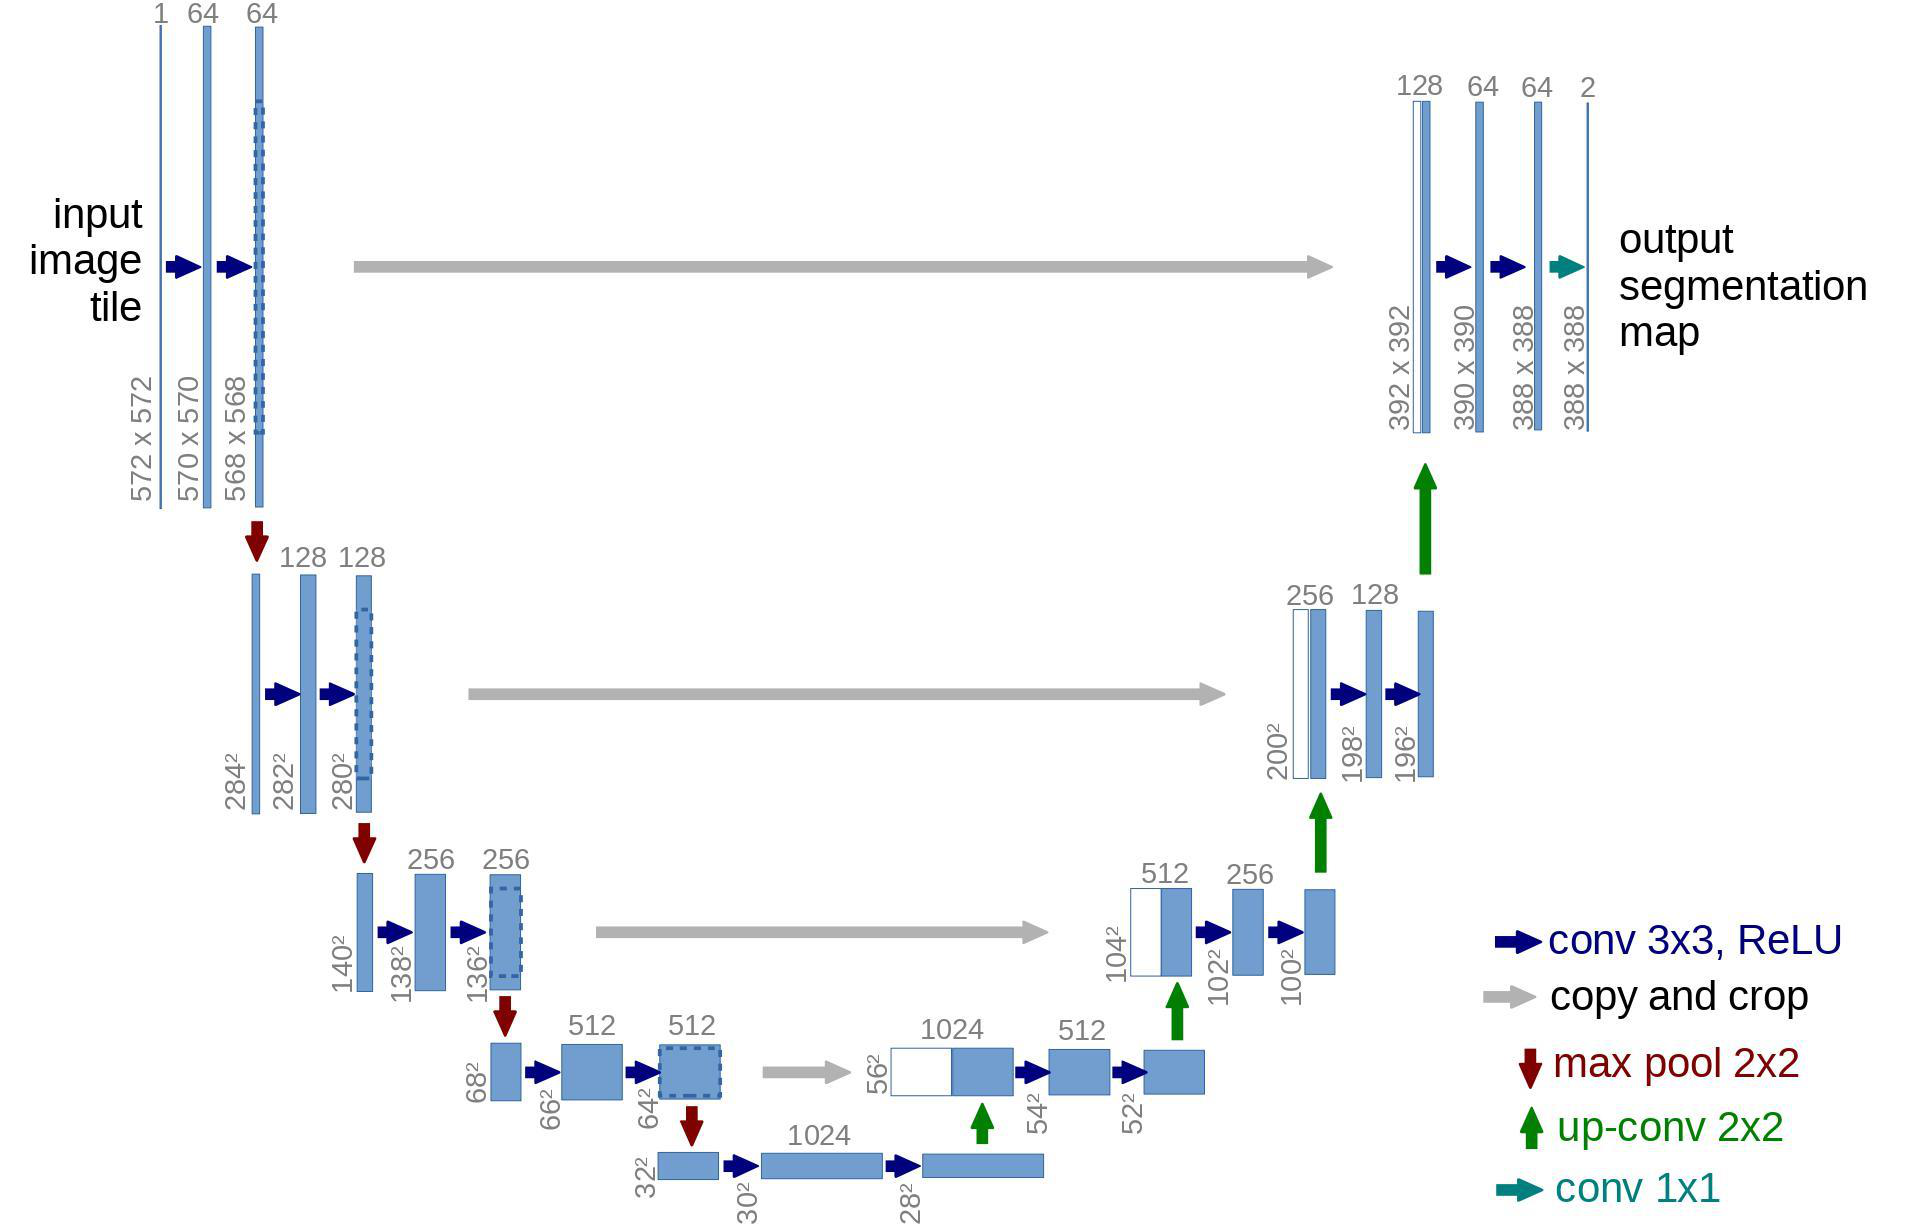
\includegraphics[width=0.8\linewidth,height=0.6\textheight,keepaspectratio]{images/stable-diffusion/unet.png}\\[0.25em]
    \binxuwSdCaption
\end{frame}


\begin{frame}{Note: Add Time Dependency}
  \begin{columns}[T,onlytextwidth]
    \column{0.54\textwidth}
    \footnotesize
    \textbf{The score function is \textit{time-dependent}.}
    \begin{itemize}
      \item[] Target: $s(x, t) = \nabla_x \log p_t(x)$, the score of the noised marginal at time $t$. It is the same object the noise predictor learns, up to a scale: $s(x,t) \approx -\epsilon_\theta(x,t)/\sigma_t$.
    \end{itemize}
    \vspace{0.7em}
    \textbf{Add time dependency}
    \begin{itemize}
      \item Assume time dependency is spatially homogeneous.
      \item Add one scalar value per channel $f(t)$.
      \item Parametrize $f(t)$ by MLP/linear of Fourier basis.
      \begin{itemize}
        \item[\hspace{0.5em}--] Fourier features: $[\sin\,\omega_i t,\, \cos\,\omega_i t,\, \ldots]$
      \end{itemize}
    \end{itemize}
    \column{0.46\textwidth}
      \centering
      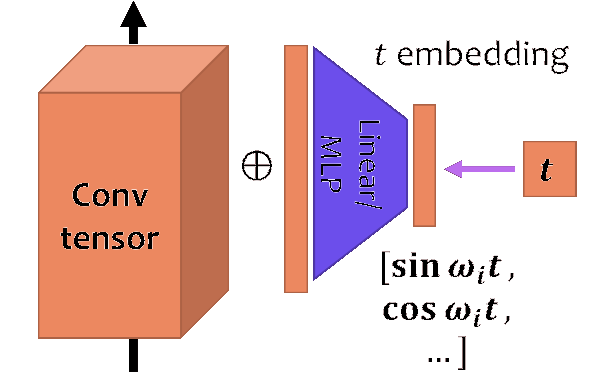
\includegraphics[width=0.96\linewidth,height=0.7\textheight,keepaspectratio]{images/stable-diffusion/add_time_dimension.png}\\[0.25em]
      \binxuwSdCaption
  \end{columns}
\end{frame}

\begin{frame}[allowframebreaks]{U-Net in Stable Diffusion}
  \begin{columns}[T,onlytextwidth]
    \column{0.44\textwidth}
      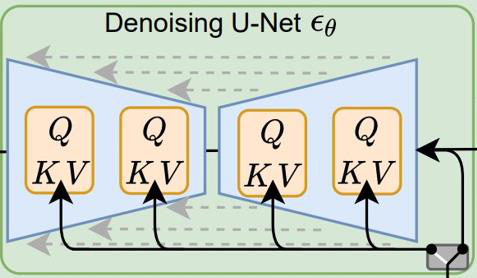
\includegraphics[width=0.99\linewidth,height=0.74\textheight,keepaspectratio]{images/stable-diffusion/attention.png}\\[0.25em]
      \binxuwSdCaption
    \column{0.56\textwidth}
      \scriptsize
      \begin{itemize}\footnotesize
        \item Input convolution: Projects 4-channel input $\rightarrow$ 320 channels using a 2D convolution.
        \item Time embedding: inject time information into the network.
        \item Downsampling: sometimes interleaved with cross-attention.
        \item Mid block: applies additional residual and (cross-)attention operations.
        \item Upsampling, normalization, activation, output convolution.
      \end{itemize} 
  \end{columns}
\end{frame}

\begin{frame}{How to Understand Prompts: Language Model Refresher}
  \begin{columns}[T,onlytextwidth]
    \column{0.48\textwidth}
      \begin{itemize}
        \item Meaning of a word depends on context, not always the same.
        \item Example: ``I \emph{book} a ticket to buy that \emph{book}.''
        \item Word vectors should depend on context.
        \item Transformers let each word absorb influence from other words to become contextualized.
      \end{itemize}
    \column{0.50\textwidth}
      \centering
      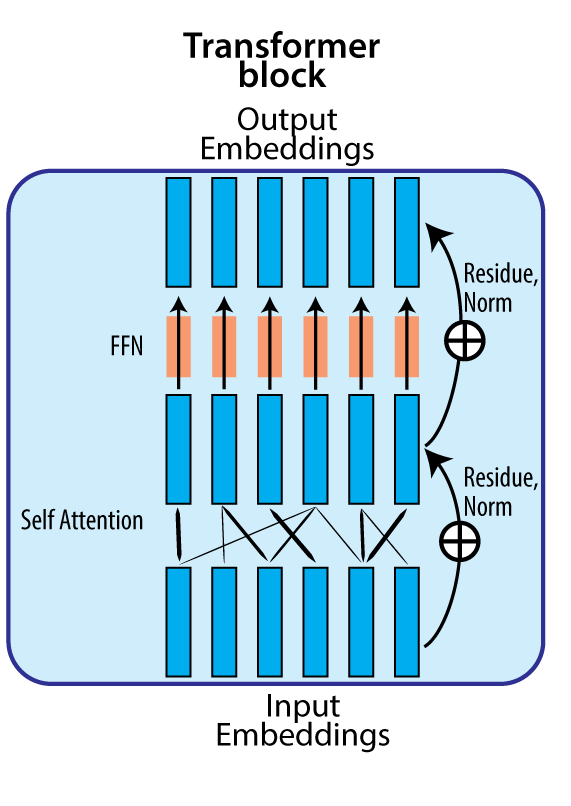
\includegraphics[width=\linewidth,height=0.72\textheight,keepaspectratio]{images/stable-diffusion/contextual_word_vectors.png}\\[0.25em]
      \binxuwSdCaption
  \end{columns}
\end{frame}

\begin{frame}{Learning Word Vectors: GPT, BERT \& CLIP}
  \begin{columns}[T,onlytextwidth]
    \column{0.48\textwidth}
      \begin{itemize}\itemsep0.35em\footnotesize
        \item Self-supervised learning of word representations.
        \item Predict missing / next words in a sentence (BERT, GPT).
        \item Contrastive learning: match image and text (CLIP).
        \item Downstream classifiers can decode part of speech, sentiment, \ldots
      \end{itemize}
    \column{0.50\textwidth}
      \centering
      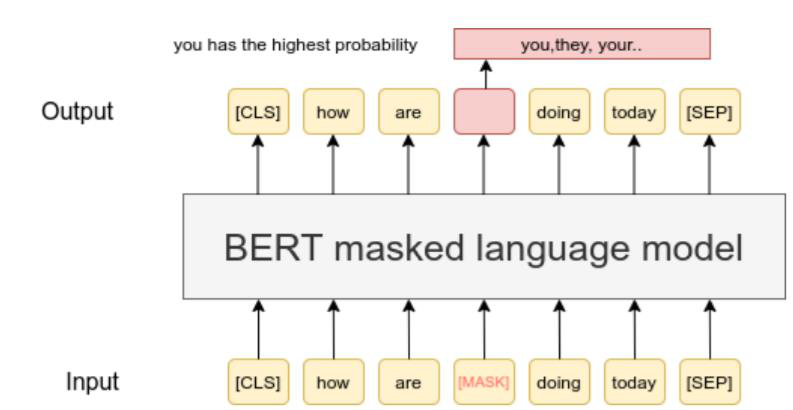
\includegraphics[width=\linewidth,height=0.72\textheight,keepaspectratio]{images/stable-diffusion/learning_word_vectors_gpt_bert_clip.png}\\[0.25em]
      \binxuwSdCaption
  \end{columns}
\end{frame}

\begin{frame}{Joint Representation for Vision and Language: CLIP}
  \begin{columns}[T,onlytextwidth]
    \column{0.48\textwidth}
      \begin{itemize}
        \item Learn a joint encoding space for text captions and images.
        \item Maximize representation similarity between an image and its caption.
        \item Minimize similarity for other pairs.
      \end{itemize}
    \column{0.50\textwidth}
      \centering
      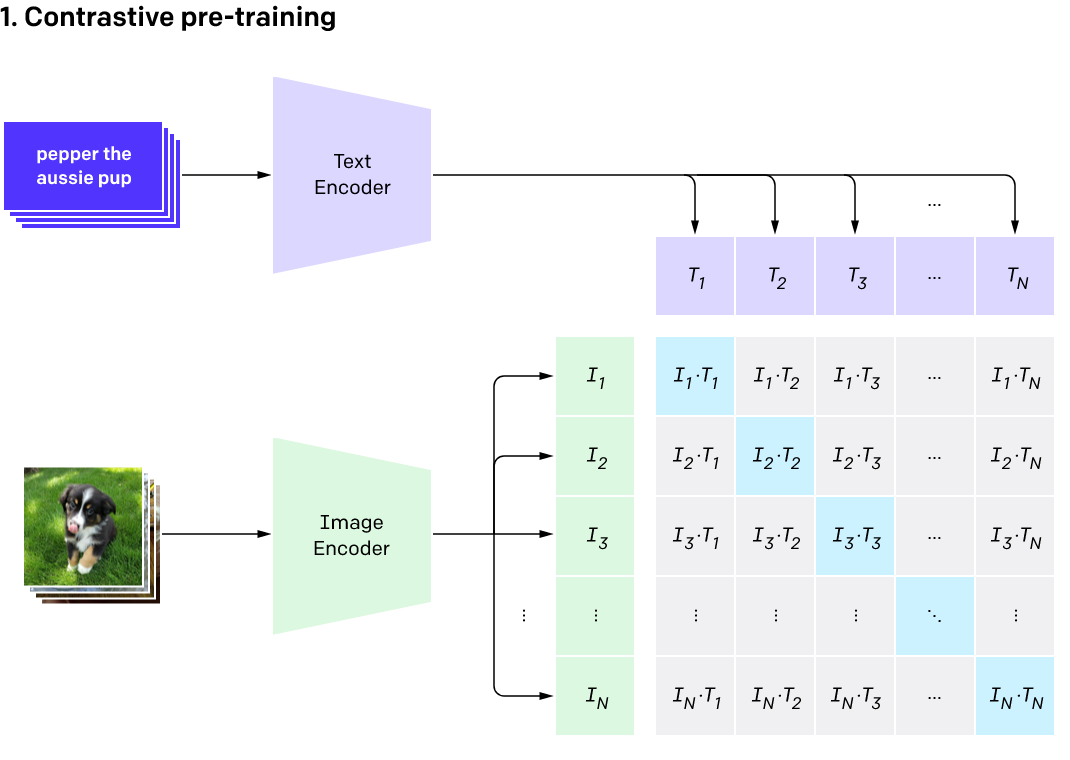
\includegraphics[width=\linewidth,height=0.72\textheight,keepaspectratio]{images/stable-diffusion/clip_joint_representation.png}\\[0.25em]
      {\scriptsize
        Adapted from: Radford et al., \href{https://arxiv.org/abs/2103.00020}{CLIP, arXiv:2103.00020}
      }
 
  \end{columns}
\end{frame}

\begin{frame}{Choice of Text Encoding}
      \begin{itemize}
        \item Encoder in Stable Diffusion v1: frozen, pre-trained CLIP ViT-L/14 text encoder. Later versions differ: SD~2 uses OpenCLIP ViT-H/14, SDXL two encoders, SD~3 adds T5-XXL.
        \item Word vectors can also be randomly initialized and learned online.
        \item \textbf{Other conditional signals:}
        \begin{itemize}
          \item Object categories (e.g.\ Shark, Trout): one vector per class.
          \item Face attributes (e.g.\ \{female, blonde hair, with glasses\}): one vector per attribute.
        \end{itemize}
        \item Time to be creative!
      \end{itemize}
\end{frame}
